\documentclass{ctexart}
    \usepackage{mathrsfs}
    \usepackage{multirow}
    \usepackage{graphicx}
    \usepackage{array}
    \usepackage{makecell}
    \usepackage{amsmath}
    \usepackage{booktabs}
    \usepackage{float}
    \usepackage{diagbox}
    \newcommand\mgape[1]{\gape{$\vcenter{\hbox{#1}}$}}
    \newcommand\Ronum[1]{\uppercase\expandafter{\romannumeral #1\relax}}
    \newcommand\ronum[1]{\romannumeral #1\relax}
    \author{钱思天\ 1600011388 No.8}
    \title{实验十五\ 非平衡电桥测量铂电阻的温度系数 \ 实验报告}
    \begin{document}
      \maketitle
      \section{实验数据与处理}
      \subsection{测量结果及作图}
      在条件:$I=4.007mA$及$R_0=100.1\Omega$下进行测量,实测数据表如下:
      % Table generated by Excel2LaTeX from sheet 'Sheet2'
\begin{table}[H]
  \centering
  \caption{实测数据$(\mbox{条件}:I=4.007mA\&R_0=100.1\Omega)$}
    \begin{tabular}{|c|c|c|c|c|c|c|c|}
      \hline
    次数$i$     & 1     & 2     & 3     & 4     & 5     & 6     & 7 \\
    \hline
    水温$T/^\circ C$     & 0.1   & 24.4  & 39.2  & 56.1  & 69.4  & 85.3  & 100.0 \\
    \hline
    $U_{out}/mV$ & 0.00  & 18.66 & 29.93 & 42.91 & 52.88 & 64.92 & 75.97 \\
  \hline  
  \end{tabular}%
  \label{tab:addlabel}%
\end{table}%

根据实测数据表作图,得下图:

\begin{figure}[H]
  \centering
  \caption{$U_{out}-T$散点及趋势线图}
  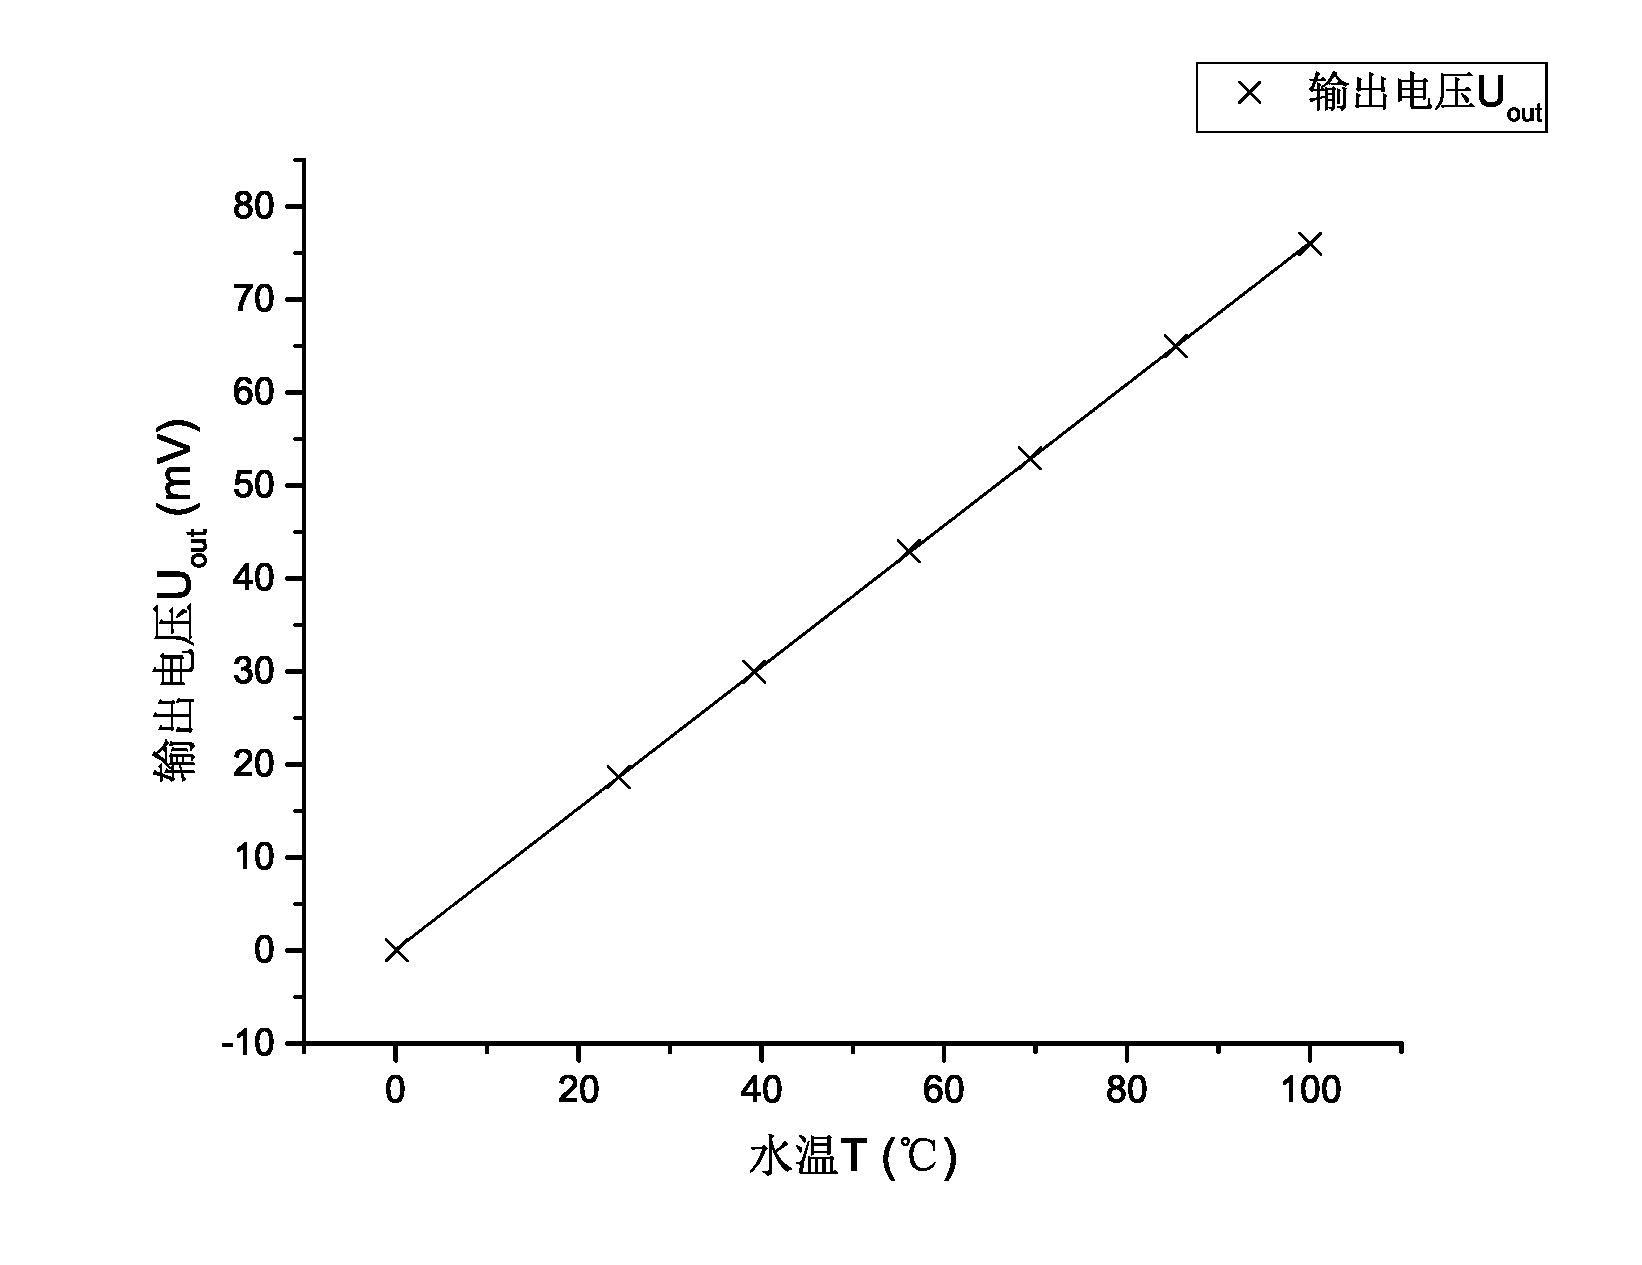
\includegraphics[width=1.0\textwidth]{1}
  \label{fig:digit}
\end{figure}

从趋势线可以看出$U_{out}$与$T$成线性关系,计算相关系数有$r^2\approx0.99996$,故确实有较强的线性相关性。
 \section{计算铂电阻的温度系数及其不确定度}
 根据公式$$U_{out}=\frac{I}2 R_0AT$$
 
 有:
 $$A=\frac{k}{R_0\frac{I}2}$$
 $$\sigma_A=\sqrt{(\frac{\partial A}{\partial k})^2\sigma_k^2+(\frac{\partial A}{\partial R_0})^2\sigma_{R_0}^2+(\frac{\partial A}{\partial \frac{I}2})^2\sigma_{\frac{I}2}^2}$$

 又其中:
$$(\frac{\partial A}{\partial \frac{I}2})^2\sigma_{\frac{I}2}^2=(\frac{k}{R_0(\frac{I}2)^2})^2\cdot \frac{(0.5\%I+0.004)^2}{3\times 2^2}=1.724\times 10^{-10}$$
$$(\frac{\partial A}{\partial R_0})^2\sigma_{R_0}^2=(\frac{k}{R_0^2\frac{I}2})^2\cdot \frac{(0.1\%R_0)^2}{3}=4.792\times 10^{-12}$$

下计算$k$的不确定度,利用最小二乘法,设$$U_{out}=k\times T+b$$
$$k=\frac{\sum\limits_{i=1}^{7}{({U_{out}}_i-\bar{U}_{out})(T_i-\bar{T})}}{\sum\limits_{i=1}^{7}{(T_i-\bar{T})^2}}=0.7604$$
$$\sigma_k=\frac{\sigma_{U_{out}}}{\sqrt{\sum\limits_{i=1}^{7}{(T_i-\bar{T})^2}}}$$

又:$$\sigma_{U_{out}}=\sqrt{\sigma_A^2+\frac{e^2}3}=\sqrt{k^2\frac{1-r^2}{7-2}+\frac{(0.05\%U_{outmax}+0.03)^2}{3}}$$

代回,得:
$$\sigma_k=\frac{\sigma_{U_{out}}}{\sqrt{\sum\limits_{i=1}^{7}{(T_i-\bar{T})^2}}}=0.001$$

即$$k\pm \sigma_k=0.760\pm0.001$$

得:
$$(\frac{\partial A}{\partial k})^2\sigma_k^2=(\frac{1}{R_0\frac{I}2})^2\cdot \sigma_k^2=4.8732\times 10^{-11}$$

故:

$$A=3.79\times 10^{-3}(^\circ C^{-1})$$
$$\sigma_A=2 \times 10^{-5}(^\circ C^{-1})$$
$$A\pm \sigma_A=(379\pm2)\times 10^{-5}(^\circ C^{-1})$$


\section{思考题}
\subsection{引起非线性误差因素及实验措施}
\paragraph{因素}大致可分为以下几点:
\subparagraph{1}桥臂电阻称不上远大于铂电阻及二桥臂电阻不相等,这就导致了在铂电阻阻值改变的过程中,$U_{out}$不线性输出。
\subparagraph{2}电桥部分存在的接触电阻,导线内阻等电阻,可能会影响到实验。
\subparagraph{3}电流的因素,要保证稳定性。
\subparagraph{4}温度范围还需要在铂电阻随温度线性变化区间内,才能保证线性输出。
\paragraph{措施}针对这些因素,可分别采取如下措施:
\subparagraph{1}使用高精度的大内阻标准电阻,完成测量。
\subparagraph{2}采用三线式接法,并注意导线的选取。
\subparagraph{3}采用稳流源,用万用表检测电流,并利用万用表电压档极高内阻特性,用万用表做电压表测量$U_{out}$。
\subparagraph{4}实验中选取水的冰点到沸点,端点稳定,且位于线性变化区域内。
\subsection{截距问题}
\paragraph{原因}我认为,一来由于温度计的测量精度问题,使得初温的读数存在偏移,同时,$R_0$也可能无法与零点电阻完全相等,从而导致截距不为零。
\paragraph{影响}我认为,对实验结果无影响。本实验中,我们更多的考虑斜率,利用斜率进行计算。当然,如果截距偏离较大,可能零点电阻未能匹配,从而使实验结果不准确的可能性也是存在的。
\section{分析与讨论}
\subsection{比较理论值与实测值}
\paragraph{现象}从数据来看,本次实验所得的实测数据,即便考虑不确定度,也仍然不能使理论值落在区间内。且实测值较理论值更小。

\paragraph{分析}我认为,原因是实验中,由于热敏电阻的改变,我们所采用的线性近似不再准确,即由于电阻增大,流经铂电阻的电流小于$\frac{I_0}{2}$,使得$U_{out}$测量值较小,故而计算时得到的温度系数数值会偏小。



\section{收获与感想}
从前,我知道平衡电桥十分巧妙。

今天,我又感受到了非平衡电桥的神奇。

通过今天的实验,我感受到了不同类型物理量相互转化的思想,从温度计到传感器,无不体现着这一思想的精妙之处。

而且,我也在老师的讲解中,对热力学量的测量精度有了大概的了解,也产生了一定的兴趣。

最重要的是,在本次的实验中,我感受到了,在平衡附近的线性近似的实际应用。这一在题目中常常涉及的方法,终于在单摆之外见到了另一个实际的例子。

在今后的实验课程中,我也会提高自己的实验能力,多想多思考,也去了解一些感觉很普通的事物的不普通的应用。




\end{document} 